\documentclass{article}
\usepackage{graphicx} % Required for inserting images
\usepackage{booktabs}
\usepackage{float}
\usepackage{multirow}
\usepackage{tabularx}
\usepackage{hyperref}
\usepackage{array}
\usepackage[a4paper, top=1.5cm, bottom=1.5cm, left=2.5cm, right=2.5cm]{geometry}

\title{Investigating the robustness and applicability of Deep RNNs}
\author{
 Petru-Theodor Cristea, Cringanu Denis-Florin\\
  Eftimie Petre-Laurentiu, Hodoroaga Andrei
}
\date{June 2025}

\begin{document}

\maketitle

\begin{abstract}
This project replicates and extends the work of Pascanu \textit{et al.}~\cite{pascanu2013construct}, 2013, on constructing deep recurrent neural networks (RNNs). We first reproduce the original architectures, including the Deep Transition RNN with shortcut connections (DT(S)-RNN), Deep Output, Deep Transition RNN with shortcut connections (DOT(S)-RNN), and the Stacked RNN (sRNN), evaluating them on the original polyphonic music and language modeling benchmarks. We then explore the hyperparameter sensitivity of these architectures, such as hidden layer size, transition layer size, and number of layers. A comparison with other similar models, GRU~\cite{cho2014learning} and LSTM ~\cite{hochreiter1997long}, is also provided. To further test the generality of these deep recurrent models, we introduce two additional datasets for word-level language modeling: the Brown Corpus~\cite{francis1979brown} and the CoNLL 2000~\cite{tjong-kim-sang-buchholz-2000-introduction} dataset. The implementation in python can be found \href{https://github.com/lowLevelGod/DeepRNNs}{here}.
\end{abstract}

\section{Introduction}

We implement several RNN architectures for sequence modeling tasks. The first architecture is a shallow RNN, serving as our baseline. To capture more dependencies, we implement the Deep Transition RNN with shortcut connections (DT(S)-RNN). This architecture deepens the hidden-to-hidden transition by inserting a multilayer perceptron, allowing the network to model more complex state transitions. We further extend this approach with the Deep Output and Transition RNN with shortcut connections (DOT(S)-RNN), which introduces multiple fully connected layers in the hidden-to-output mapping. Another architecture, the Stacked RNN (sRNN), enables hierarchical sequence processing, where upper layers can model more abstract temporal features based on the representations formed by lower layers. In addition, the LSTM and GRU architectures are used for further comparison. Finally, we provide a gradient flow analysis to observe how the deep RNNs compare to the shallow RNNs.

For word-level text modeling tasks, each architecture is further adapted with a trainable embedding layer that transforms discrete tokens into dense vector representations, facilitating semantic understanding. These adapted models preserve the original RNN architecture and integrate dropout where necessary to mitigate overfitting.


\section{Training and Hyperparameter Sensitivity}

Training on the polyphonic music modeling datasets was conducted using Stochastic Gradient Descent (SGD)\cite{bottou2012stochastic} with exponential learning rate decay and gradient clipping, following the methodology established in the original work by Pascanu et al. (2013). In contrast, for the language modeling datasets, the ADAM\cite{kingma2014adam} optimizer (Kingma \& Ba, 2014) was employed to facilitate more stable and efficient convergence.
Due to computational constraints, the number of training epochs was fixed for all experiments. Across both task categories, Binary Cross Entropy Loss with logits (BCEWithLogitsLoss\cite{bcewithlogitsloss}) was used as the primary loss function to ensure numerical stability when handling probabilistic multi-label outputs. In addition to the loss, accuracy was also monitored and reported as a secondary performance metric to provide complementary insights into the models' predictive effectiveness.


To evaluate model robustness, we performed a sensitivity analysis for each architecture by systematically varying key hyperparameters, including hidden size, model depth, transition size, and number of layers (specifically for the Stacked RNN). We also conducted experiments using standard recurrent units such as vanilla RNN~\cite{elman1990finding}, Long Short-Term Memory (LSTM), and Gated Recurrent Unit (GRU). The vanilla RNN captures sequential dependencies using a simple recurrent structure but struggles with long-range dependencies due to vanishing gradients. LSTM addresses this by introducing memory cells and gating mechanisms that regulate the flow of information over time. GRU offers a simplified alternative to LSTM by combining the forget and input gates into a single update gate.


\section{Datasets Summary}

We evaluate sequence modeling architectures on two categories of datasets: polyphonic music and part-of-speech (POS) tagged text corpora.

For the polyphonic music domain, we utilize three piano-roll formatted datasets. The \textbf{Nottingham}\cite{boulanger2012modeling} dataset comprises British and American folk tunes, primarily featuring monophonic melodies accompanied by simple harmonic structures. The \textbf{MuseData}\cite{museData} corpus contains complex classical music scores spanning a range of composers and instruments, offering rich polyphonic textures. The \textbf{JSB Chorales}\cite{boulanger2012modeling} dataset consists of four-part harmonizations by Johann Sebastian Bach and is widely regarded in symbolic music modeling tasks.

For POS-tagged text modeling, we employ three annotated corpora. The \textbf{Penn Treebank}~\cite{marcus1993building} serves as a benchmark dataset. The \textbf{Brown Corpus} includes a balanced selection of English texts from a variety of genres. The \textbf{CoNLL-2000} dataset contains POS-tagged sentences using the IOB (Inside-Outside-Beginning) annotation format and spans a wide range of textual domains.


\section{Experiments}

\subsection{Gradient Flow Analysis}

We implement comprehensive gradient monitoring to capture gradient norms during backpropagation across sequence lengths of 10-200 timesteps and varying architectural depths, enabling systematic analysis of vanishing and exploding gradient phenomena.

Using synthetic datasets with random input sequences $\mathbf{X} \in \mathbb{R}^{32 \times T \times 10}$ where $T$ varies from 10 to 200, we isolate architectural effects on gradient flow independent of data characteristics. Our analysis reveals DT(S)-RNN consistently maintains gradient norms of 0.06-0.24 across all conditions, demonstrating superior gradient flow compared to sRNN (0.02-0.05) and DOT(S)-RNN (0.03-0.05). While no architecture exhibits technical gradient vanishing ($< 10^{-6}$) or explosion ($> 10.0$), DT(S)-RNN's 3-8x higher gradient norms translate to dramatically improved learning dynamics, providing empirical evidence for deep transition advantages over traditional stacking approaches. Figure~\ref{fig:gradient_heatmap} illustrates these gradient flow differences across all tested architectural depths and sequence lengths on a log scale, with DT(S)-RNN consistently demonstrating better gradient propagation compared to the sRNN and DOT(S)-RNN architectures.

Validation on the MuseData corpus of classical compositions confirms that our synthetic findings transfer to structured real-world data. DT(S)-RNN maintains better gradient flow with average norms of 0.0379 versus sRNN's 0.0313 on musical sequences. Notably, structured musical data exhibits more stable gradients than synthetic data (DT(S)-RNN: 0.0379 vs 0.0058), suggesting inherent temporal structure provides beneficial learning signals that complement deep transition architectural advantages. This validates our gradient analysis extends beyond controlled conditions to practical sequence modeling tasks.

\begin{figure}[ht]
    \centering
    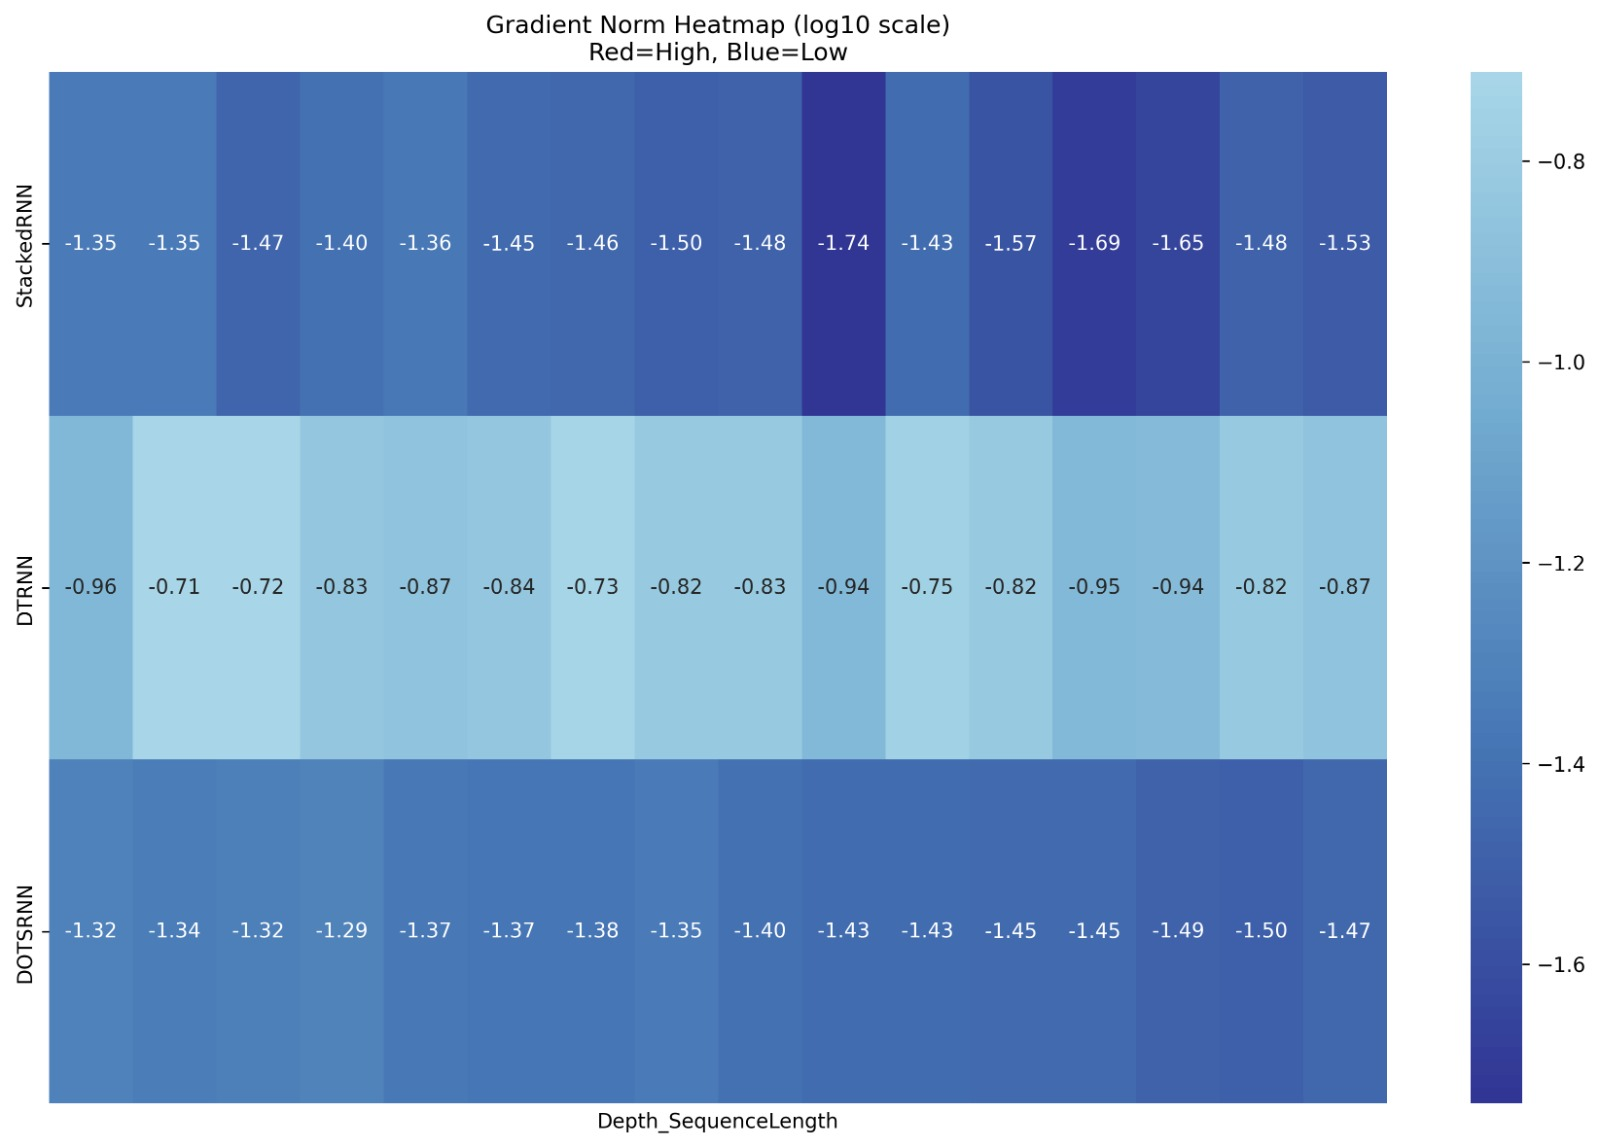
\includegraphics[width=0.8\textwidth]{Gradient Flow Analysis/gradient_flow.jpeg}
    \caption{Gradient Flow Analysis.}
    \label{fig:gradient_heatmap}
\end{figure}

\subsection{Text Modeling Datasets}

We trained simple RNN models with different hidden sizes (\texttt{hidden\_size} = 100 to 600) for 7 epochs on a character-level setup using the Treebank dataset. Across all configurations, increasing the hidden size generally led to consistent improvements in training accuracy.

\begin{figure}[H]
    \centering
    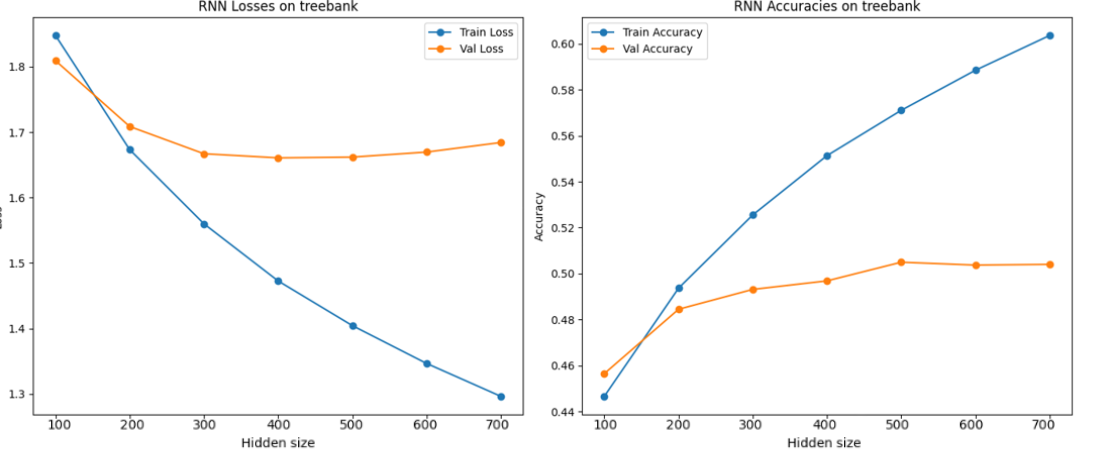
\includegraphics[width=0.8\textwidth]{treebank_charlevel_plots/rnn_hiddensize_treebank_charlevel_RIGHT_LABEL.png}
    \caption{RNN hidden size tuning on Treebank Char-Level}
    \label{fig:RNN Hidden Size tuning}
\end{figure}


We trained DT(S)-RNN models with varying recurrence depths from 2 to 8. The best validation performance was observed for \textbf{depth = 2}, reaching 37.10\% accuracy. Deeper models showed diminishing returns, with training plateauing at around 19.5\% accuracy starting from depth 5. 

\begin{figure}[H]
    \centering
    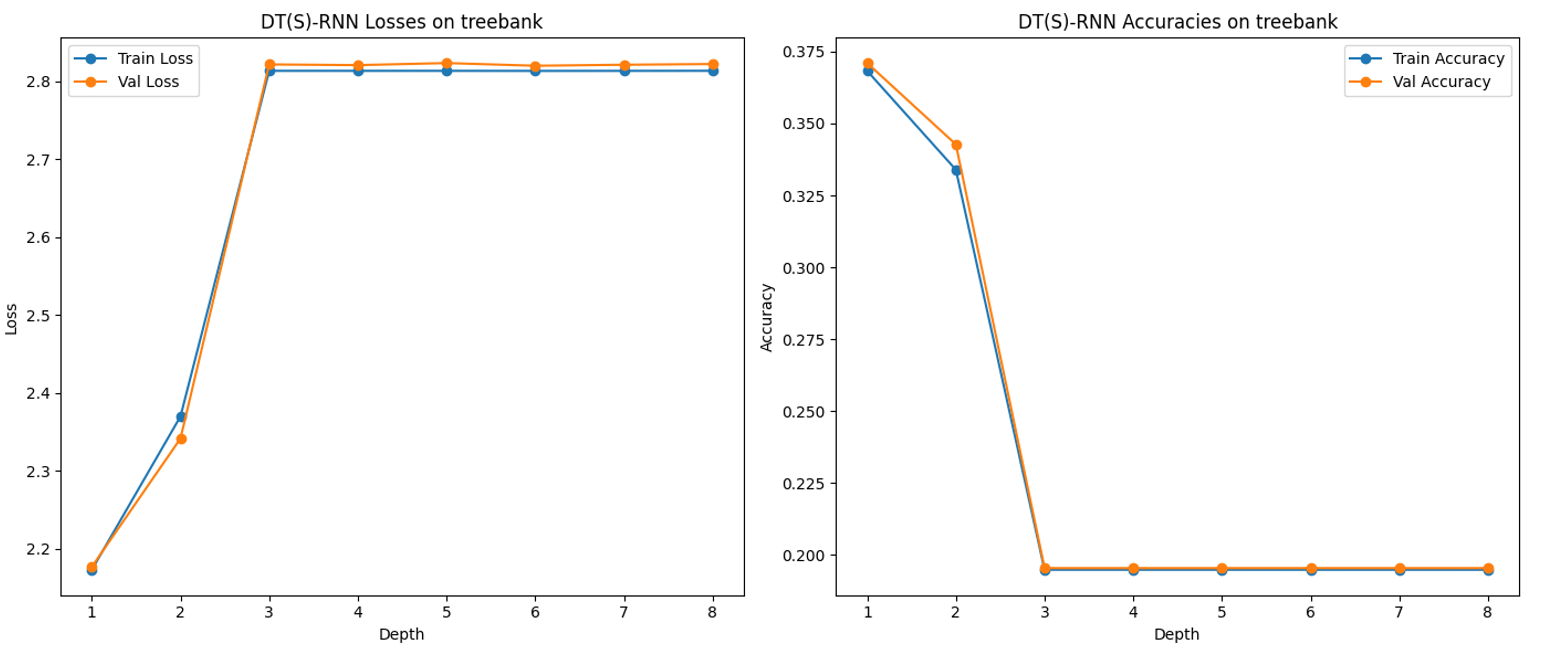
\includegraphics[width=0.8\textwidth]
    {treebank_charlevel_plots/dtsrnn_depth_treebank_charlevel.png}
    \caption{DT(S)-RNN depth tuning on Treebank Char-Level}
    \label{fig:DT(S)-RNN depth tuning}
\end{figure}


We conducted a grid search to evaluate the effect of different \texttt{transition\_size} values on DT(S)-RNN performance for the Treebank word-level task. The hidden size and recurrence depth were fixed at 200 and 3, respectively. We observed that training loss and accuracy remained relatively stable across configurations, showing minimal sensitivity to \texttt{transition\_size}.

\begin{figure}[H]
    \centering
    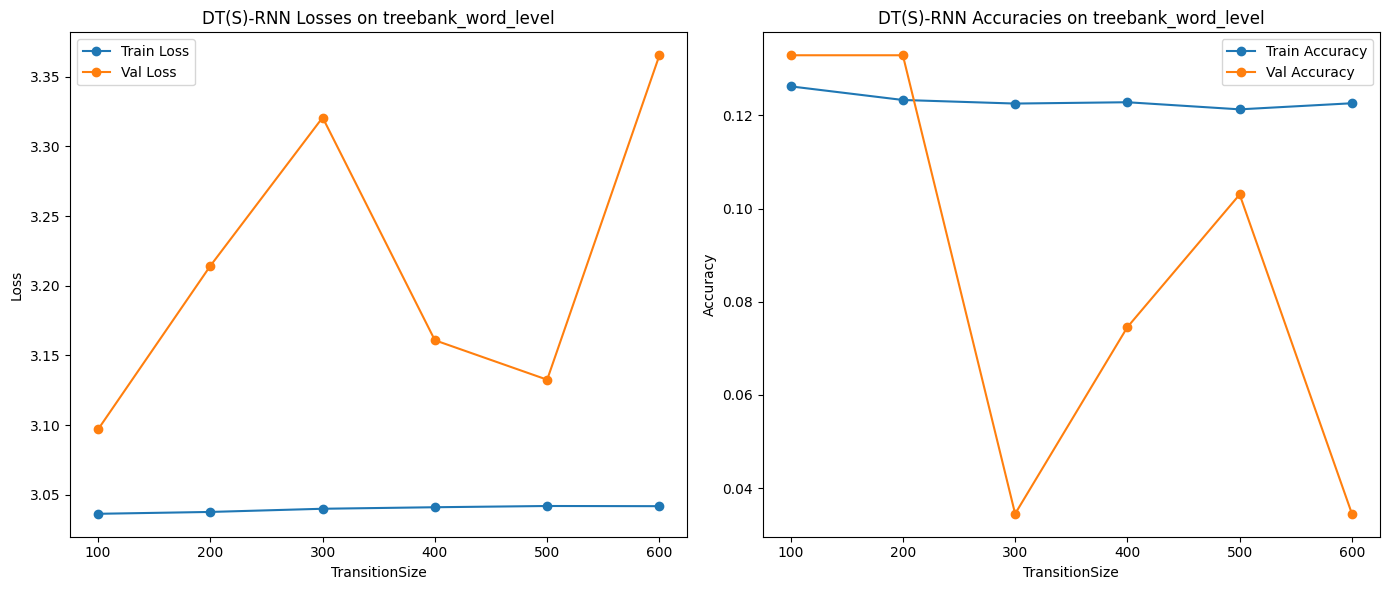
\includegraphics[width=0.8\textwidth]{treebank_wordlevel_plots/dtsrnn_transitionsize_treebank_wordlevel.png}
    \caption{DT(S)-RNN transition size tuning Treebank Word-Level}
    \label{fig:dtsrnn-transition-size-tuning}
\end{figure}


We evaluated the impact of different hidden sizes on sRNN performance for the Treebank word-level task, keeping the number of layers fixed at 2. The hidden size was varied from 200 to 700. We observed a consistent improvement in training accuracy as the hidden size increased. However, validation accuracy exhibited non-monotonic behavior, indicating that larger hidden sizes do not necessarily lead to better generalization.


\begin{figure}[H]
    \centering
    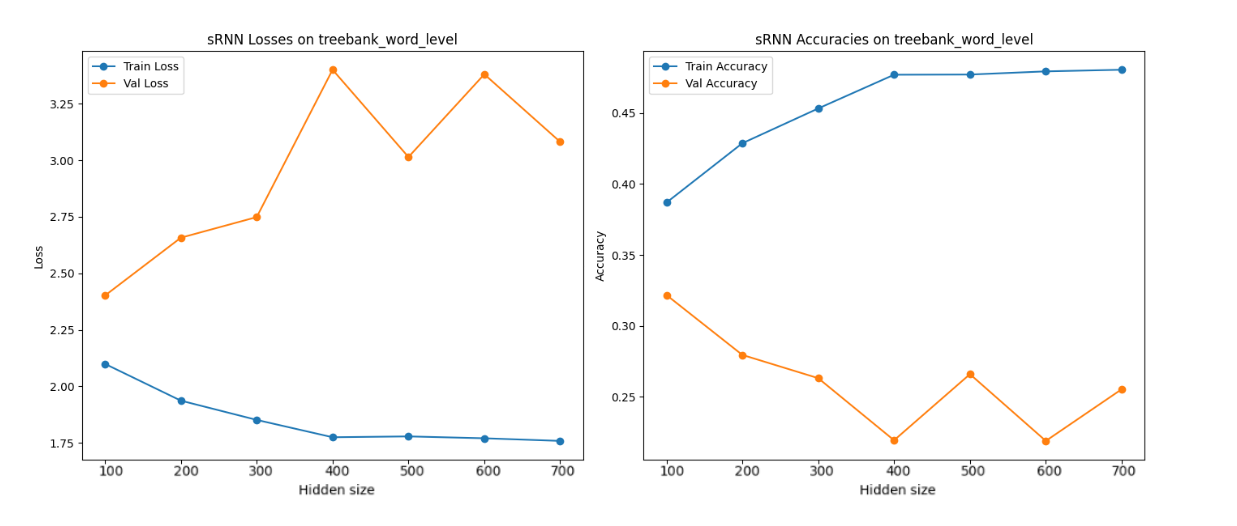
\includegraphics[width=0.8\textwidth]{treebank_wordlevel_plots/srnn_hiddensize_treebank_wordlevel_RIGHT_LABEL.png}
    \caption{sRNN hidden size tuning Treebank Word-Level}
    \label{fig:srnn-hidden-size-tuning}
\end{figure}

The table below compares the validation loss of four RNN-based architectures—RNN, DT(S)-RNN, DOT(S)-RNN, and sRNN—across varying hidden sizes on the Penn Treebank word-level task. Among all configurations, the sRNN with a hidden size of 100 achieved the lowest validation loss (2.4016), indicating superior generalization compared to both the standard RNN and the more complex transition-based models.

\begin{table}[H]
\centering
\begin{tabular}{|c|c|c|c|c|}
\hline
\textbf{Hidden Size} & \textbf{RNN} & \textbf{DT(S)-RNN} & \textbf{DOT(S)-RNN} & \textbf{sRNN} \\
\hline
100 & 2.4248 & 3.1010 & 8.7786 & \textbf{2.4016} \\
200 & 2.7130 & 3.1098 & 8.6688 & 2.6574 \\
300 & 3.2689 & 3.2481 & 8.5965 & 2.7487 \\
400 & 2.4264 & 3.1890 & 8.5561 & 3.4005 \\
500 & 2.6061 & 3.3677 & 8.5288 & 3.0144 \\
600 & 2.5255 & 3.1871 & 8.5130 & 3.3805 \\
700 & 2.6507 & 3.1907 & 8.4992 & 3.0814 \\
\hline
\end{tabular}
\caption{Validation loss at epoch 7 for different models and hidden sizes on the Penn Treebank word-level task. Best (lowest) value overall in bold.}
\label{tab:val_loss_table}
\end{table}


The results in the plot below demonstrate that increasing the depth of the DT(S)-RNN model beyond 2 layers does not improve performance on the given dataset. The shallowest model (depth = 2) achieves the best validation accuracy of 32.33\%, with a corresponding validation loss of 1.9419. Deeper models (depths 3, 5, 6, 7, and 8) show a notable drop in validation accuracy, often around 10.56\%, suggesting potential overfitting or difficulty in training deeper architectures with the current hyperparameters. 

\begin{figure}[H]
    \centering
    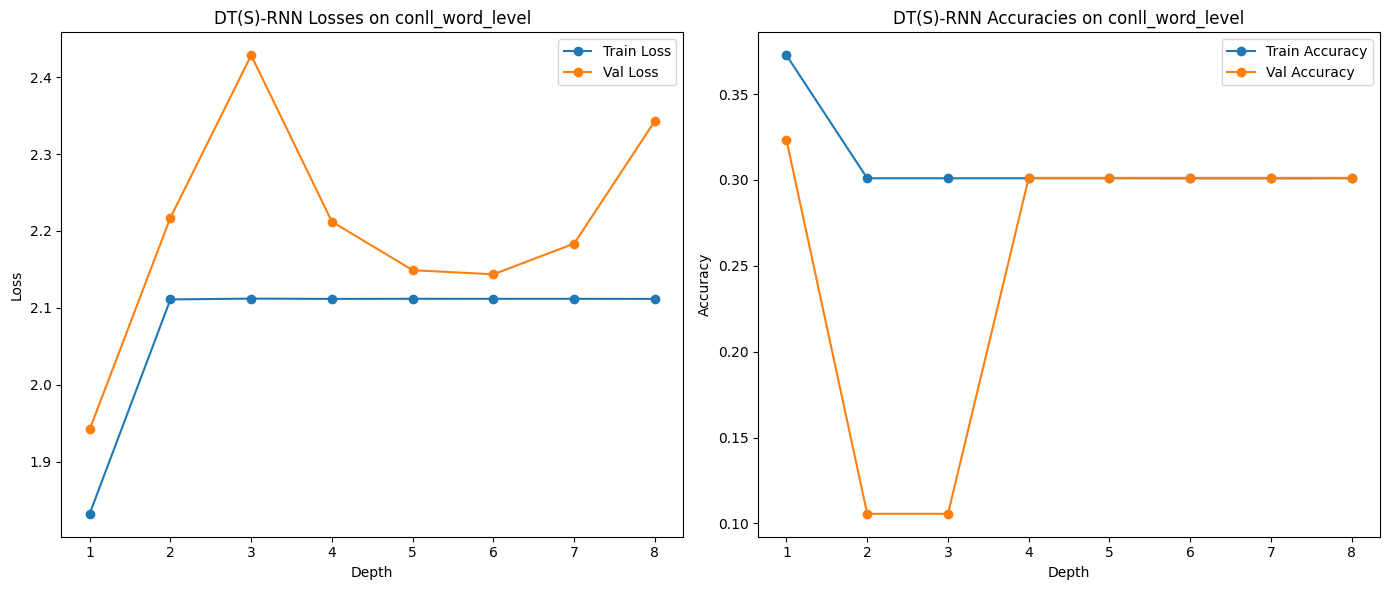
\includegraphics[width=0.8\textwidth]{conll_wordlevel_plots/dtsrnn_depth_conll_wordlevel.png}
    \caption{DT(S)-RNN depth tuning ConLL Word-Level}
    \label{fig:srnn-hidden-size-tuning}
\end{figure}

 In this plot it is presented the training and validation performance of the DT(S)-RNN model with varying hidden sizes, while keeping the transition size fixed at 200 and depth at 3. As the hidden size increases from 100 to 700, both training and validation accuracies generally improve. The highest validation accuracy (35.17\%) is observed at a hidden size of 300, with a validation loss of 1.8454. However, beyond this size, the validation accuracy fluctuates and does not show a consistent increase. 

\begin{figure}[H]
    \centering
    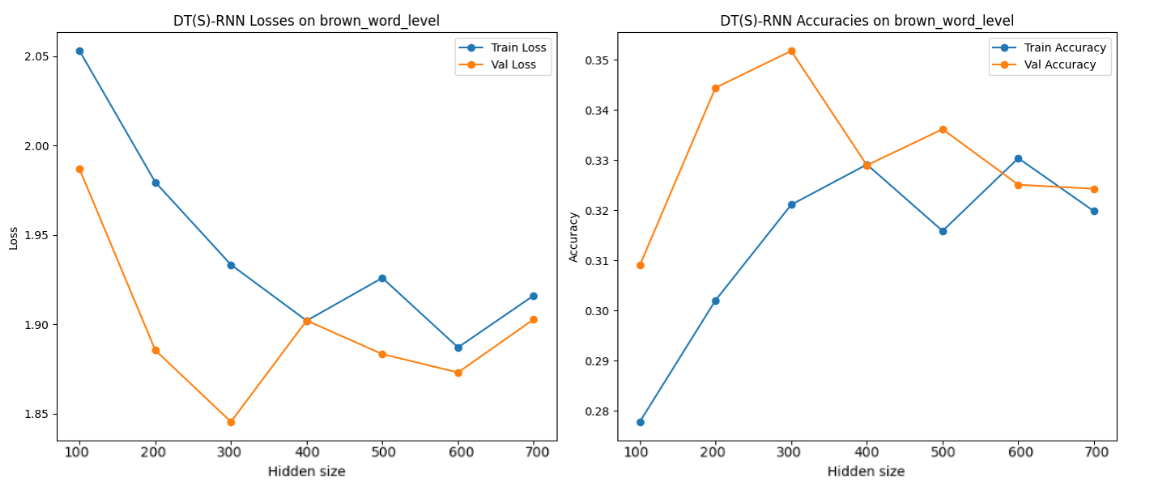
\includegraphics[width=0.8\textwidth]{brown_plots/dtsrnn_hiddensize_brown_wordlevel_RIGHT_LABEL.png}
    \caption{DT(S)-RNN depth tuning ConLL Word-Level}
    \label{fig:srnn-hidden-size-tuning}
\end{figure}

\subsection{Polyphonic Music Datasets}

We observed a higher performance across all the models on these datasets and also a lower training time, probably due to the simplicity of the data. All the tests below were done by fixing all the hyperparameters with the value $200$ for layer size hyperparameters and $2$ for depth and number of layers hyperparameters, except one, for which the search was performed using values from the set 
$\{10, 50, 100, 150,200, 400, 600\}$ for layers size and $\{2,3, 4, 5,6, 7, 8\}$ for the rest. Training was done for 10 epochs on each model configuration and each dataset due to computational restrictions.

\begin{figure}[H]
    \centering
    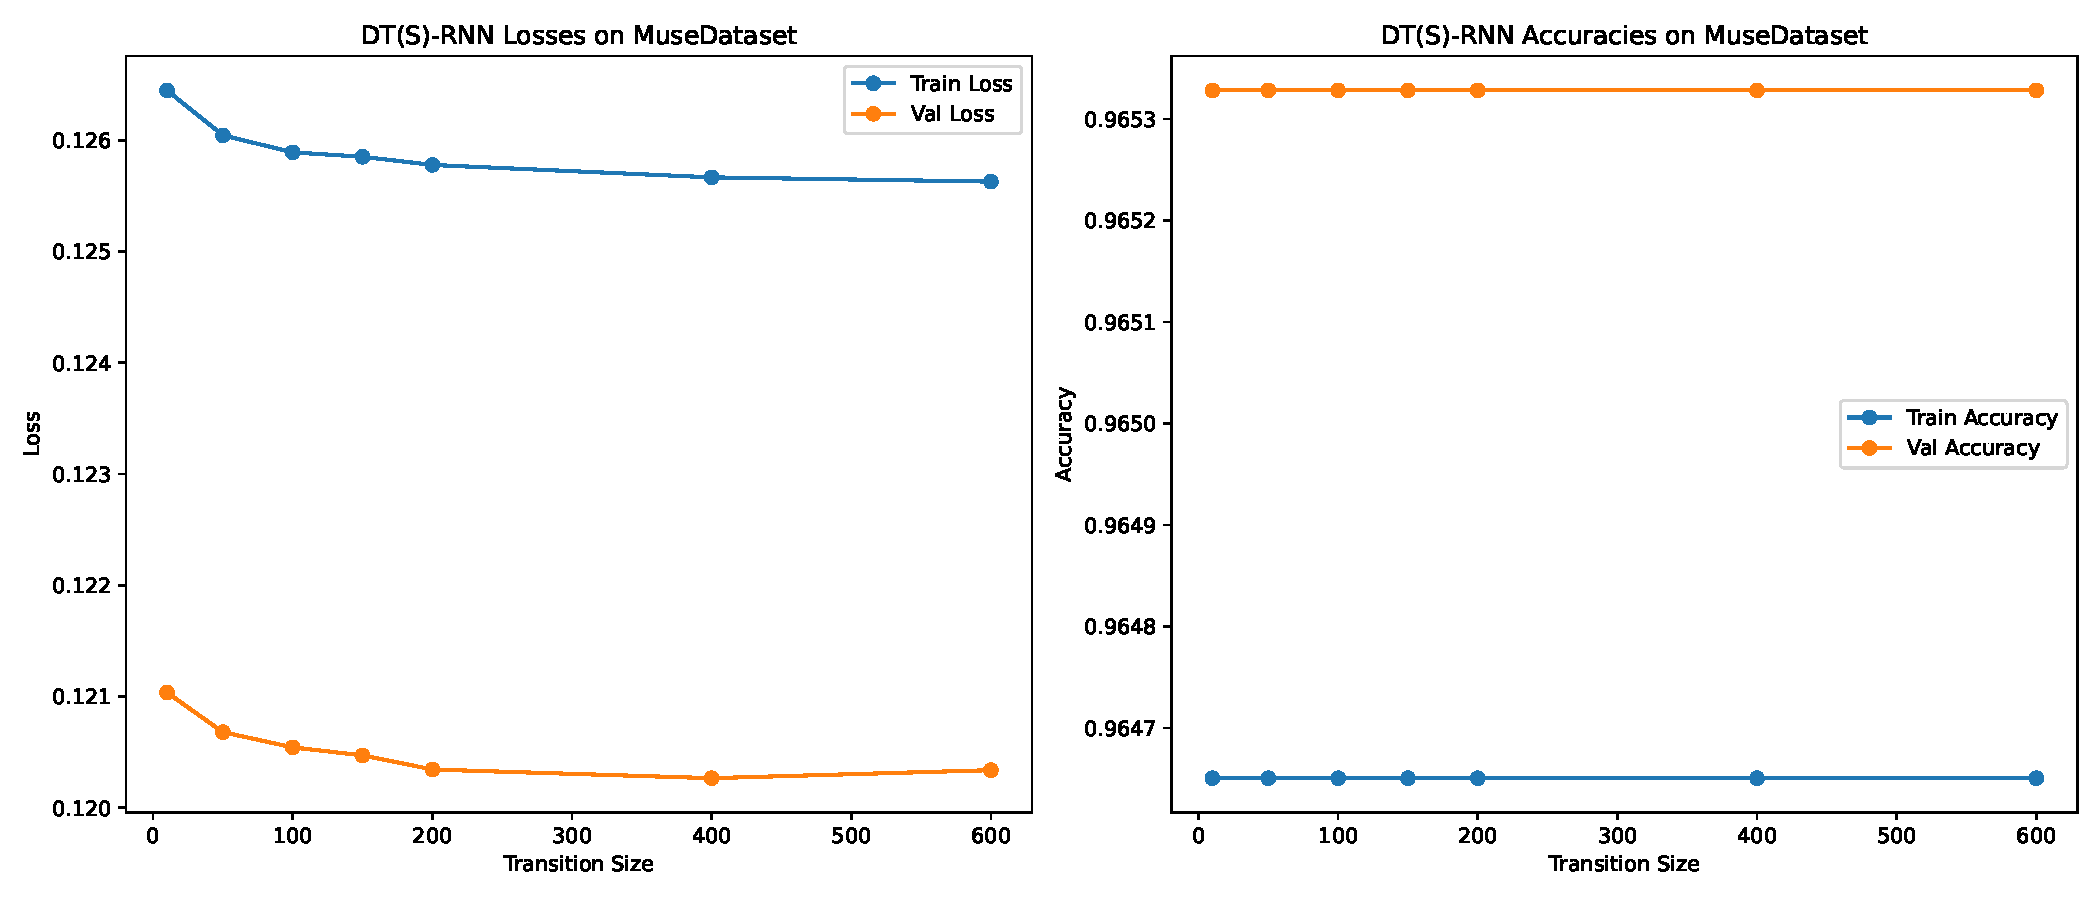
\includegraphics[width=0.8\textwidth]{Muse/DT(S)-RNN_MuseDataset_transition_sizes_comparison.pdf}
    \caption{DT(S)-RNN transition size tuning on Muse Dataset.}
    \label{fig:dts-transition-size-tuning-muse}
\end{figure}

For all models, increasing the \textbf{hidden size} resulted in improved performance until around 400 hidden size, after which it started to saturate.
Higher values of \textbf{transition size} mostly increased DT(S)-RNN's performance, while for DOT(S)-RNN, no significant improvement could be observed and even lower values for transition size gave a similar result to higher ones.

\begin{figure}[H]
    \centering
    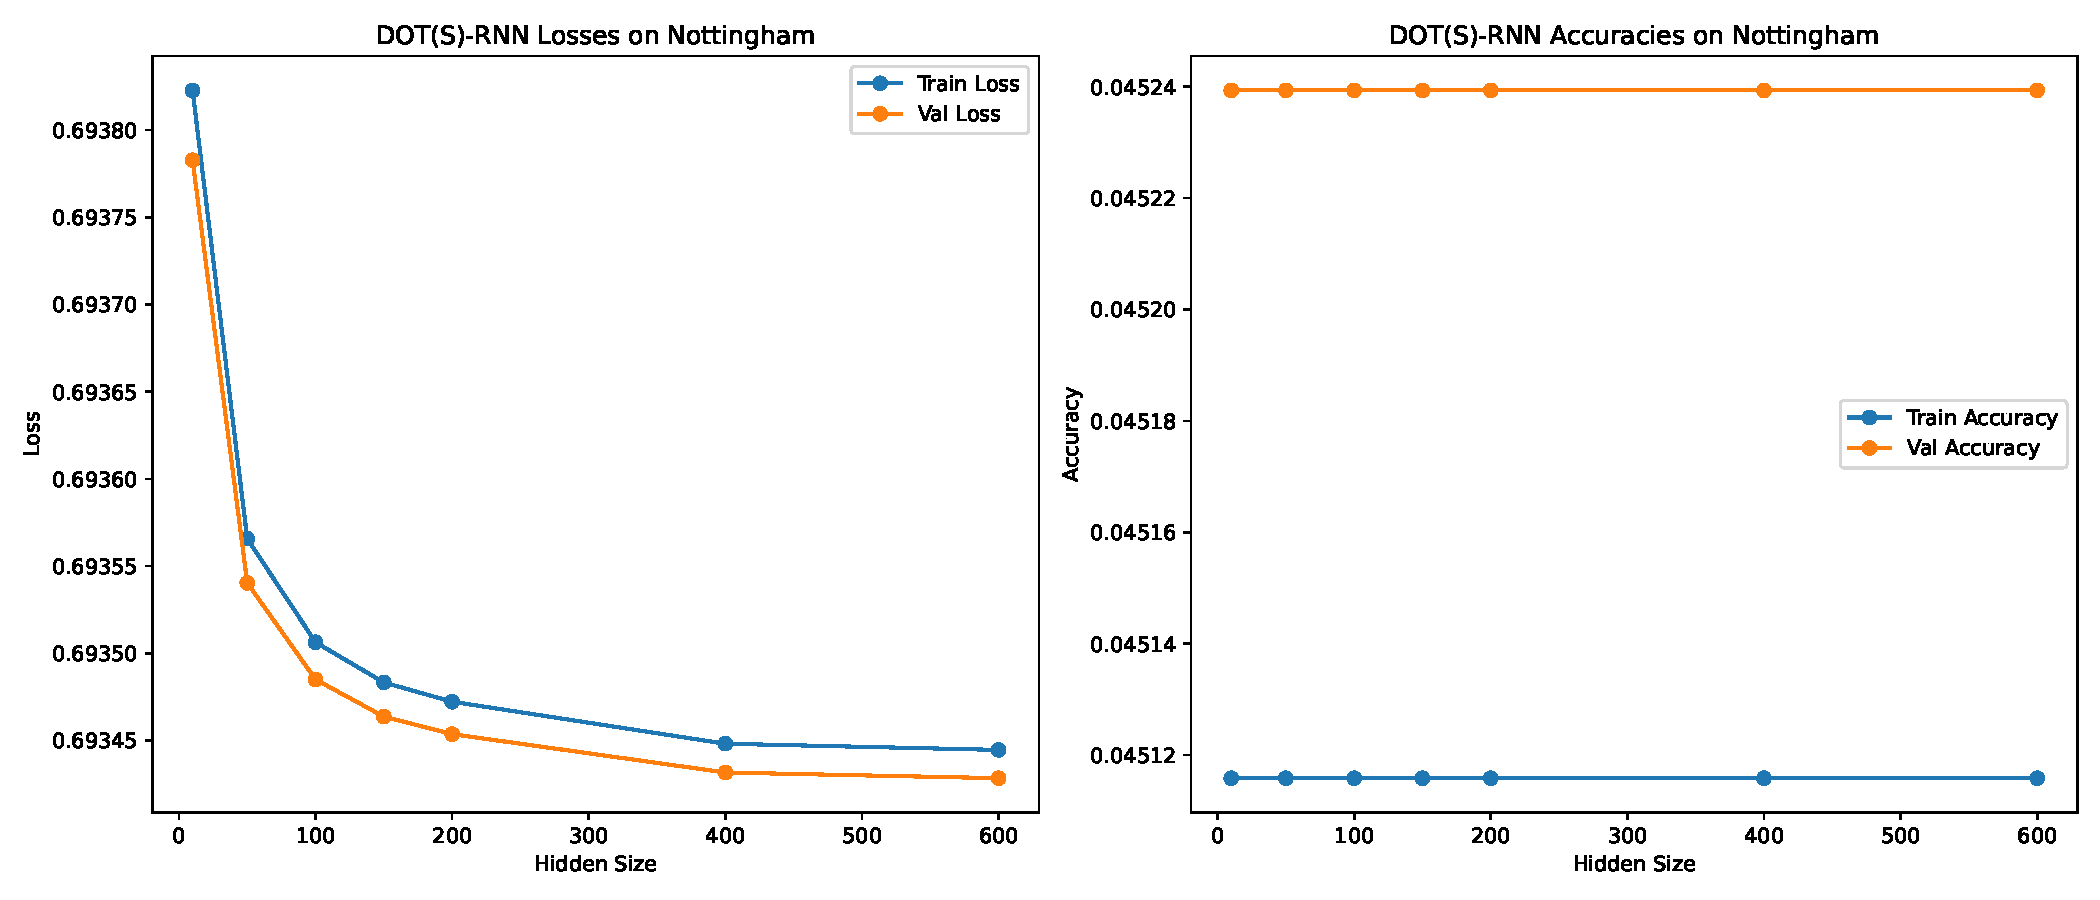
\includegraphics[width=0.8\textwidth]{Nottingham/DOT(S)-RNN_Nottingham_intermediate_output_sizes_comparison.pdf}
    \caption{DOT(S)-RNN intermediate output size variation Nottingham Dataset.}
    \label{fig:dots-intermediate-output-size-tuning-Nottingham}
\end{figure}

The \textbf{intermediate output size} of the DOT(S)-RNN greatly reduced the loss using higher values.
Using more \textbf{layers} for the sRNN, LSTM and GRU cases made the performance worse on the JSB Chorales and Nottingham datasets, whilst having little to no impact on the Muse dataset.
Neither increasing nor decreasing the \textbf{depth} of the transition layer or the depth of the output layer had a significant impact upon the performance of the models. 

\begin{figure}[H]
    \centering
    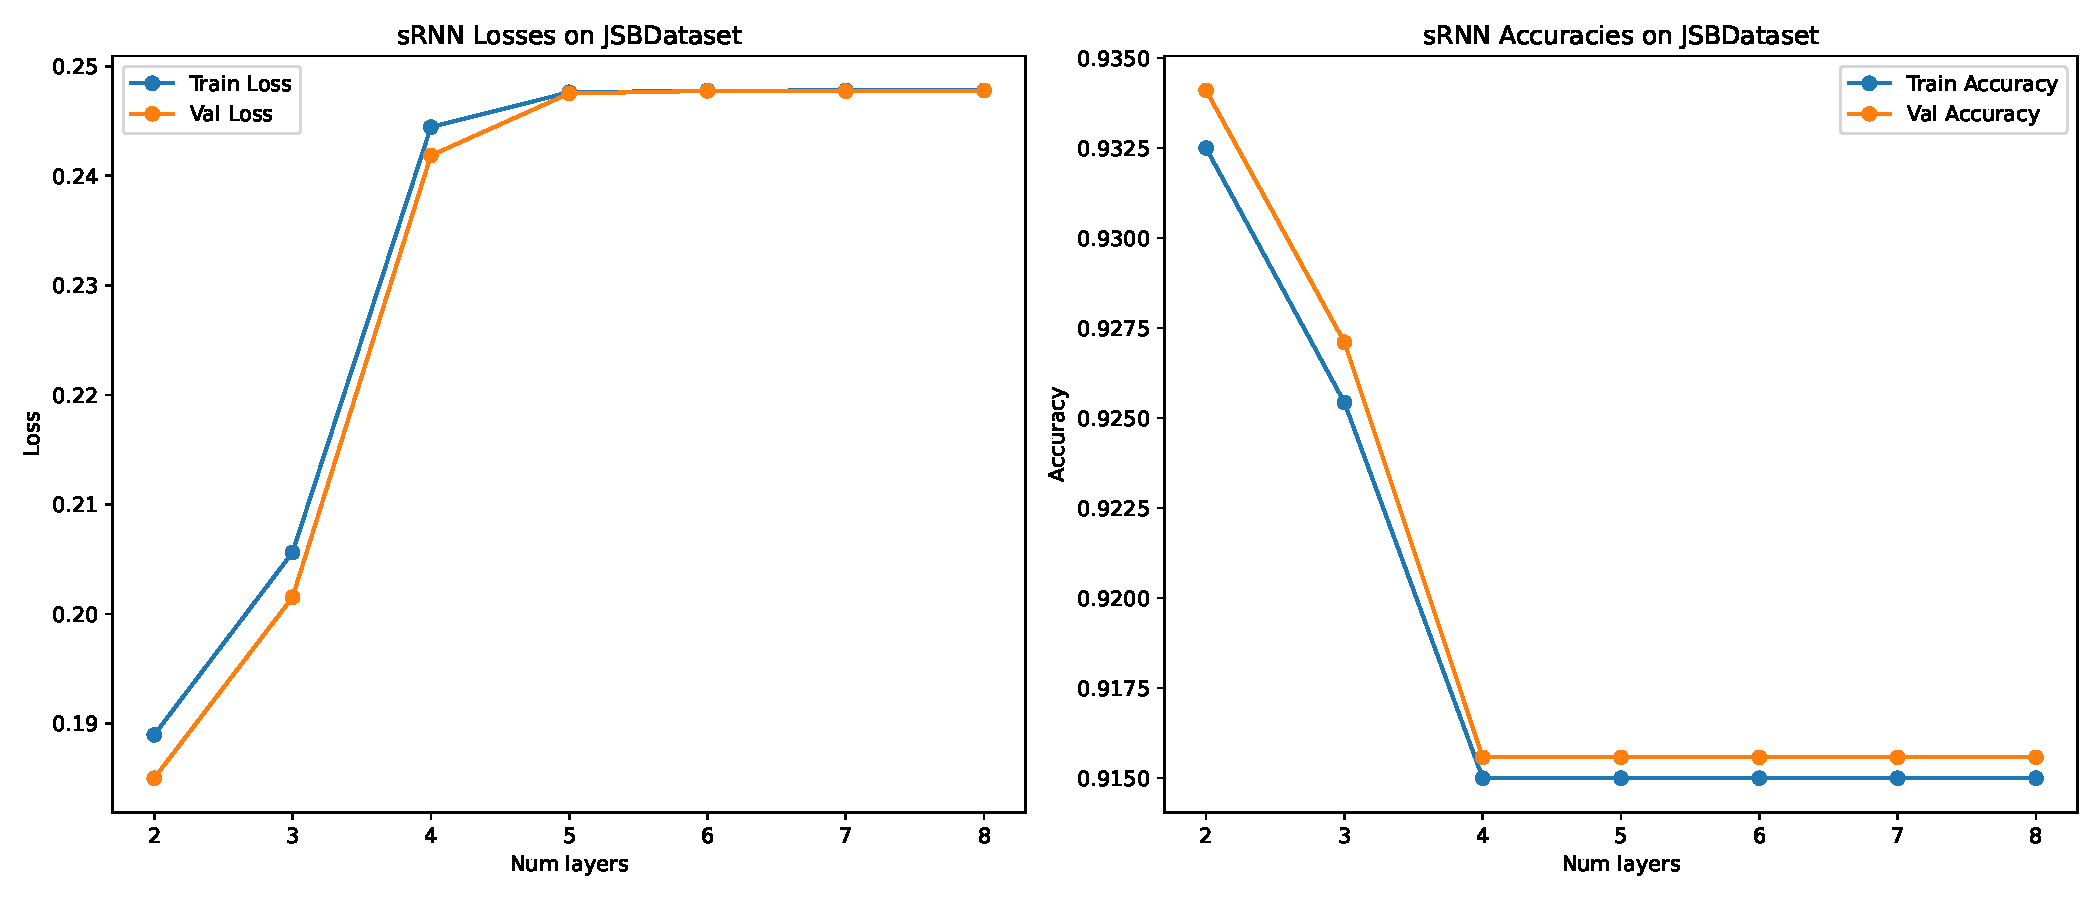
\includegraphics[width=0.8\textwidth]{JSB/sRNN_JSBDataset_num_layers_comparison.pdf}
    \caption{sRNN number of layers tuning on JSB Chorales Dataset.}
    \label{fig:srnn-num-layers-tuning-jsb}
\end{figure}

Table below shows validation loss at epoch 10 across RNN-based models with varying hidden sizes on the JSB Chorales dataset.
\begin{table}[H]
\centering
\small
\begin{tabularx}{\textwidth}{|c|X|X|X|X|X|X|}
\hline
\textbf{Hidden Size} & \textbf{RNN} & \textbf{DT(S)-RNN} & \textbf{DOT(S)-RNN} & \textbf{sRNN} & \textbf{LSTM} & \textbf{GRU} \\
\hline
10  & 0.2479 & 0.2486 & 0.7001 & 0.2484 & 0.2486 & 0.2495 \\
50  & 0.2105 & 0.2477 & 0.6947 & 0.2294 & 0.2406 & 0.2110 \\
100 & 0.1903 & 0.2477 & 0.6940 & 0.2040 & 0.2341 & 0.1998 \\
150 & 0.1785 & 0.2477 & 0.6938 & 0.1927 & 0.2394 & 0.1955 \\
200 & 0.1741 & 0.2477 & 0.6937 & 0.1802 & 0.2323 & 0.1930 \\
400 & 0.1667 & 0.2477 & 0.6935 & 0.1672 & 0.2336 & 0.1900 \\
600 & \textbf{0.1616} & 0.2477 & 0.6935 & 0.1602 & 0.2331 & 0.1896 \\
\hline
\end{tabularx}
\caption{Validation loss for different models and hidden sizes on JSB Chorales.}
\label{tab:jsb_val_loss_table}
\end{table}

\section{Conclusion}
This study demonstrates that DT(S)-RNNs maintain superior gradient flow, enhancing learning stability across long sequences. Hyperparameter tuning revealed diminishing returns beyond moderate hidden sizes and depths. Overall, deep transition architectures offer benefits, but simplicity can outperform under constrained settings.

\clearpage
\bibliographystyle{plain}
\bibliography{references}

\end{document}
